\documentclass[11pt, oneside]{article} 
\usepackage{geometry}
\geometry{letterpaper} 
\usepackage{graphicx}
	
\usepackage{amssymb}
\usepackage{amsmath}
\usepackage{parskip}
\usepackage{color}
\usepackage{hyperref}

\graphicspath{{/Users/telliott_admin/Dropbox/Tex/png/}}
% \begin{center} 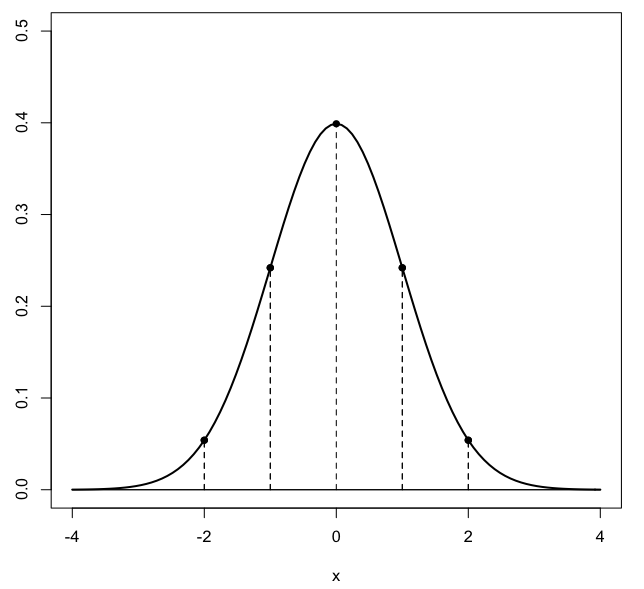
\includegraphics [scale=0.4] {gauss3.png} \end{center}

%break
\title{Logarithmic differentiation}
\date{}

\begin{document}
\maketitle
\Large

Now that we know the definition
\[ \ln x = \int \frac{1}{x} \ dx + C \]
by the fundamental theorem of calculus:
\[ \frac{d}{dx} \ln x = \frac{1}{x} \]

We can extend this to a general $f(x)$ using the chain rule
\[ \frac{d}{dx} \ln (f(x)) = \frac{1}{f(x)} \ f'(x) \]
Rearrange:
\[ \frac{f'(x)}{f(x)} = (\ln (f(x))' \]
or
\[ \frac{y'}{y} =  \ [ \ln y ]' \]

Check this with a simple example
\[ y = x^2 \]
\[ y' = 2x \]
\[ 2x = x^2 \ [ \ \ \frac{d}{dx} \ln x^2 \ ] \]
\[ 2x = x^2 \ [ \  \frac{1}{x^2} \ 2x \ ] \]

\subsection*{Slightly different statement}
Write
\[ y = f(x) \]
\[ \ln y = \ln f(x) \]

Now differentiate implicitly.  Imagine that $x$ (and $y$) are functions of $t$ and differentiate with respect to $t$.  By the chain rule:
\[ \frac{1}{y} \ \frac{dy}{dt} = \frac{1}{f(x)} \ f'(x) \ \frac{dx}{dt} \]
Lose the $dt$:
\[ \frac{1}{y} \ dy = \frac{1}{f(x)} \ f'(x) \ dx \]
\[ (\ln y)' = \frac{1}{f(x)} \ f'(x) \]

This is a slight variation of what we had above.  We can see that it works by a bit of manipulation.  We had
\[ \frac{1}{y} \ dy = \frac{1}{f(x)} \ f'(x) \ dx \]
\[ \frac{1}{y} \ dy = \frac{1}{y} \ y' \ dx \]
\[ \frac{1}{y} \ \frac{dy}{dx} = \frac{1}{y} \ y'  \]
\[ \frac{dy}{dx} = y'  \]
But of course.

\subsection*{example}

A new problem using this result is to find the derivative of $x^x$, where the standard methods don't work.  

Take the logarithm:
\[ \ln (x^x) = x \ln x \]
Now, take the derivative of the logarithm of $f(x)$:
\[ 1 \cdot \ln x + x \cdot \frac{1}{x} = \ln x + 1 \]

Use the rule:
\[ y' = y  \ \frac{d}{dx} \ln y \]
\[ = x^x \  (\ln x + 1) \]

\subsection*{example}

In general, any time we have a power of x that is itself a function, we need logarithmic differentiation.

\[ y = x^{\cos x} \]
\[ \ln y = \cos x \ln x \]
\[ \frac{1}{y} \ dy = \ [ \ \frac{\cos x}{x} - \sin x \ln x \ ] \ dx \]
\[ \frac{dy}{dx} = x^{\cos x} \ [ \ \frac{\cos x}{x} - \sin x \ln x \ ]  \]

\subsection*{power rule}

An important result is to prove the power rule for all real $x$.  We want
\[   \frac{d}{dx} x^n \]

where $n$ is not just a positive or negative integer ($\ne -1$), but can be any real number, like $\pi$ or $e$ or $\sqrt{2}$.  Straight-up implicit differentiation is easier for all but the irrational numbers, but it's a subtle thing to talk about real numbers as the limits of rational numbers.  We combine logarithmic and implicit differentiation

Write
\[ y = x^n \]
\[ \ln y = n \ \ln x \]

Imagine both $x$ and $y$ as functions of $t$ with $x = t$, then
\[ \frac{d}{dt} \ \ln y = \frac{d}{dt} \  n \ \ln x \]

But $n$ is now \emph{just a constant} so
\[ \frac{d}{dt} \ \ln y =  n \frac{d}{dt} \ \ln x \]
\[ \frac{1}{y} \ \frac{dy}{dt} = n  \frac{1}{x} \ \frac{dx}{dt} \]
\[ \frac{1}{y} \ dy = n  \frac{1}{x} \ dx \]
\[ \frac{dy}{dx} = n  \frac{y}{x} \]
\[  = n  \frac{x^n}{x} \]
\[ = n  x^{n-1} \]

Did you see what just happened!  We proved the power rule for real $n$ in a few simple lines.  Wow.

\subsection*{example}

\[   \frac{d}{dx} x^{e} = e \ x^{e - 1}  \]
\[   \frac{d}{dx} x^{\pi} = \pi \ x^{\pi - 1}  \]

\subsection*{example}

The following problem is an example of turning calculus into arithmetic, an approach in high school courses which I really dislike.  But it's really common to see such problems there so we might as well do one.

Differentiate
\[ y = \frac{x^5}{(1-10x)\sqrt{x^2+2}} \]

We could use the product, quotient and chain rules for this (and we can be sure it will be messy in the end).  An alternative is to use the properties of the logarithm to break the right-hand side into a polynomial.  Our formula from above was
\[ \frac{y'}{y} =  \ [ \ln y ]' \]

Take the logarithm of both sides for the problem
\[ \ln y = \ln (\frac{x^5}{(1-10x)\sqrt{x^2+2}} ) \]
\[   \ln y = \ln(x^5) - \ln(1-10x) - \ln(\sqrt{x^2+2}) \]

Now, when we differentiate, it is really implicit differentiation.  The three terms are
\[  \frac{1}{x^5} 5x^4 \ dx  = \frac{5}{x} \ dx \]

\[ -\frac{1}{(1-10x)} (-10) \ dx = \frac{10}{(1-10x)} \ dx \]

\[  - \frac{1}{\sqrt{x^2+2}} \cdot \frac{1}{2\sqrt{x^2+2}} 2x \ dx = - \frac{x}{x^2 + 2}  \ dx \]

On the left we get (including the $dx$ from the terms on the right-hand side):
\[  \frac{1}{y} \frac{dy}{dx} = \frac{y'}{y} \]
\[  =   \frac{5}{x} + \frac{10}{(1-10x)} - \frac{x}{x^2 + 2} \]

To finish the problem, we need to multiply through by $y$
\[  y' = (\frac{x^5}{(1-10x)\sqrt{x^2+2}}) ( \frac{5}{x} + \frac{10}{(1-10x)} - \frac{x}{x^2 + 2}) \]

which I won't try to simplify.

\end{document}